\documentclass[border=3pt]{standalone}
% Shared by the independently buildable vector figures.
\usepackage[T1]{fontenc}
\usepackage{amsmath,amssymb,newpxtext,newpxmath}
\usepackage[semibold]{sourcesans}
\usepackage{pgfplots}
\pgfplotsset{compat=1.18}
\usetikzlibrary{arrows.meta,calc,positioning}
\usepgfplotslibrary{groupplots}
\definecolor{ink}{HTML}{19303A}
\definecolor{sea}{HTML}{00675E}
\definecolor{clay}{HTML}{A24725}
\definecolor{muted}{HTML}{4C636C}
\definecolor{rulegray}{HTML}{CAD4D4}
\definecolor{wash}{HTML}{EAF4F0}
\definecolor{warm}{HTML}{F7EEE5}
\color{ink}
\tikzset{every picture/.style={font=\sffamily\small},
  arrow/.style={-{Stealth[length=2mm]},line width=.8pt,draw=muted}}
\pgfplotsset{companion/.style={axis lines=left,axis line style={draw=muted},
  tick style={draw=muted},ticklabel style={font=\sffamily\footnotesize,text=muted},
  label style={font=\sffamily\small},grid=major,grid style={draw=rulegray!64,line width=.25pt},
  tick align=outside,enlarge x limits=false,scaled ticks=false,
  every axis plot/.append style={line join=round},
  legend style={draw=none,fill=none,font=\sffamily\footnotesize},
  title style={font=\sffamily\bfseries\small,anchor=south west,at={(0,1.03)}}}}

\begin{document}
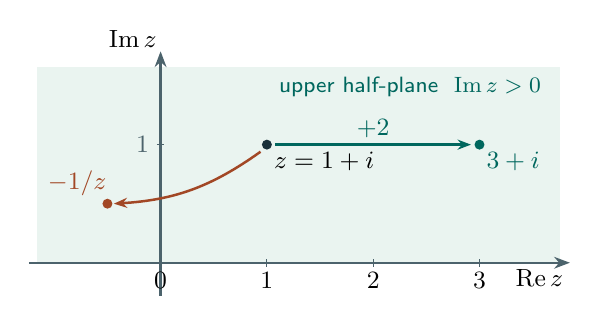
\begin{tikzpicture}[x=1.35cm,y=1.50cm,
  move/.style={-{Stealth[length=1.7mm]},line width=.9pt}]
\fill[wash] (-1.16,0) rectangle (3.76,1.66);
\draw[arrow] (-1.24,0)--(3.85,0) node[below left,inner sep=2pt] {$\operatorname{Re}z$};
\draw[arrow] (0,-.28)--(0,1.79) node[above left,inner sep=1pt] {$\operatorname{Im}z$};
\node[anchor=east,text=sea,font=\sffamily\footnotesize] at (3.67,1.49)
  {upper half-plane \ $\operatorname{Im}z>0$};
\foreach \x in {0,1,2,3}{
  \draw[muted] (\x,-.035)--(\x,.035);
  \node[below,inner sep=1.5pt] at (\x,-.04) {$\x$};
}
\draw[muted] (-.035,1)--(.035,1) node[left=2pt] {$1$};
\draw[move,sea] (1.08,1)--(2.92,1)
  node[midway,above,inner sep=2pt,text=sea] {$+2$};
\draw[move,clay] (.94,.94) to[bend left=16] (-.44,.50);
\fill[ink] (1,1) circle (1.8pt);
\fill[sea] (3,1) circle (1.8pt);
\fill[clay] (-.5,.5) circle (1.8pt);
\node[anchor=north west,inner sep=2.4pt] at (1,1) {$z=1+i$};
\node[anchor=north west,inner sep=2.4pt,text=sea] at (3,1) {$3+i$};
\node[anchor=south east,inner sep=1.3pt,text=clay] at (-.47,.53) {$-1/z$};
\end{tikzpicture}
\end{document}
